\documentclass[11pt]{scrartcl}

\title{Systemtest}
\author{Silvan Adrian \\ Fabian Binna}
\date{\today{}}

\usepackage[ngerman]{babel}
\usepackage[automark]{scrpage2}
\usepackage[colorlinks = true,
linkcolor = black]{hyperref}
\usepackage{color}
\usepackage[normalem]{ulem}
\usepackage{scrpage2}
\usepackage{graphicx}
\usepackage{tabularx}
\graphicspath{ {../../../22_Grafiken/01_Logo/}{images/}{../images/Sprint3/}{../../22_Grafiken/01_Logo/} }
\pagestyle{scrheadings}

\clearscrheadfoot
\ihead{
\includegraphics[scale=0.3]{SDDC}}
\ohead{Projekt: SDDC}
\ifoot{Systemtest}
\cfoot{Version: 1.00}
\ofoot{Datum: 23. November 2015}
\setheadsepline{0.5pt}
\setfootsepline{0.5pt}

\usepackage{ucs}
\usepackage[utf8]{inputenc}
\usepackage[T1]{fontenc}


\begin{document}
\def\arraystretch{1.5}
\begin{titlepage}
\begin{center}
\vspace{10em}

\includegraphics[scale=2]{SDDC}
\vspace{10em}
\end{center}
\begin{center}
\huge {Testprotokoll}\\
\huge {07.12.15 - Sprint 3}\\
\end{center}
\begin{center}
\vspace{10em}
\LARGE {Silvan Adrian} \\
\LARGE {Fabian Binna}
\end{center}

\end{titlepage}


\newpage
\tableofcontents
\newpage

\section{Test}
\subsection{Angaben zum Test}

\begin{tabularx}{\linewidth}{l l l}
\textbf{datum des Builds} & \textbf{Tester} & \textbf{datum der Testdurchführung}\\
\hline
07.12.15 & Silvan Adrian & 07.12.15

\end{tabularx}

\subsection{Zusammenfassung Ergebnis}
\begin{tabularx}{\linewidth}{l l l}
\textbf{Test durchgeführt?} & \textbf{Tests erfolgreich?} & \textbf{Tests fehlgeschalgen?}\\
\hline
40 (alle) & 40 (alle) & 0 \\
\hline
\end{tabularx}


\subsection{Ergebnisse Tests}
\begin{tabularx}{\linewidth}{X l l}
\textbf{Was} & \textbf{Ok? / nicht OK?} & \textbf{Aufgetretene Fehler}\\
\hline
\textbf{Unit-Tests} & {\color{green} OK}  & keine\\
\hline
Systemtest 1: & & \\
\textbf{Service abonnieren} & {\color{green} OK} & keine\\
\hline
Systemtest 2: & & \\
\textbf{OrderedService kündigen} & {\color{green} OK}  & keine\\
\hline
Systemtest 3: & & \\
\textbf{Abonnierte Services anzeigen} & {\color{green} OK}  & keine\\
\hline
Systemtest 4: & & \\
\textbf{Verfügbare Services anzeigen} & {\color{green} OK}  & keine\\
\hline
Systemtest 5: & & \\
\textbf{ServiceModul bearbeiten} & {\color{green} OK}  & keine\\
\hline
Systemtest 6: & & \\
\textbf{ServiceModul erstellen} & {\color{green} OK}  & keine\\
\hline
Systemtest 6: & & \\
\textbf{ServiceModul löschen} & {\color{green} OK}  & keine\\
\hline
Systemtest 7: & & \\
\textbf{Service bearbeiten} & {\color{green} OK}  & keine\\
\hline
Systemtest 8: & & \\
\textbf{Service erstellen} & {\color{green} OK}  & keine\\
\hline
Systemtest 9: & & \\
\textbf{Service lschen} & {\color{green} OK}  & keine\\
\hline


\end{tabularx}

\newpage

\section{Metriken}
Die abschliessenden Metriken vom Sprint aus SonarQube.
\subsection{Projekt in Zahlen}
%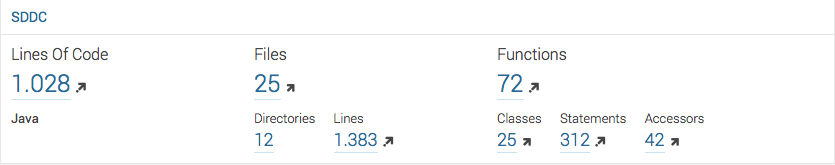
\includegraphics[width=\textwidth]{loc}

\subsection{Unit Tests Coverage}
%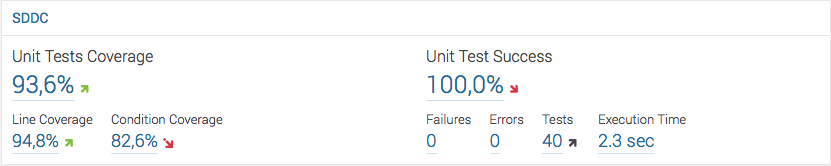
\includegraphics[width=\textwidth]{coverage}

\subsection{Coverage Verteilung auf einzelne Dateien}
%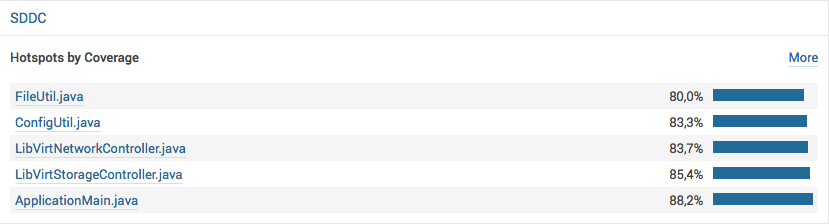
\includegraphics[width=\textwidth]{coverageperfile}

\subsection{Findbugs Issues}
%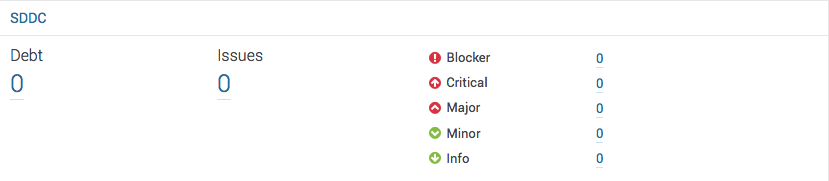
\includegraphics[width=\textwidth]{issues}
\subsubsection{Issues}
\textbf{Incorrect Lazy Initialization}
\newline
Es handelt sich hierbei um ein Multithreading Problem, welches zulassen könnte 
das der Singleton mehrmals instanziert wird, da wir bisher noch keine bessere 
Möglichkeit gefunden haben um zwischen einzelnen ConnectionStrings zu 
unterscheiden wurde es so gelöst, im nächsten Sprint wird das Problem jedoch behoben.
\newline
%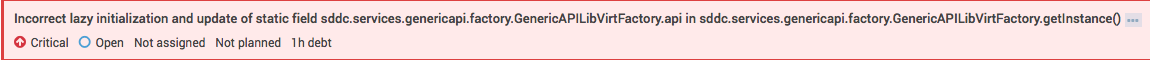
\includegraphics[width=\textwidth]{lazy}

\section{Kommentare}

Die Abschliessende App bietet nun ein Admin Dashboard, mit welchem 
Services/Servicemodule
verwaltet werden können und so bestehende Services/Servicemodule gelöscht/bearbeitet oder ganz 
neue Services/Servicemodule erstellt werden.
\newline
% 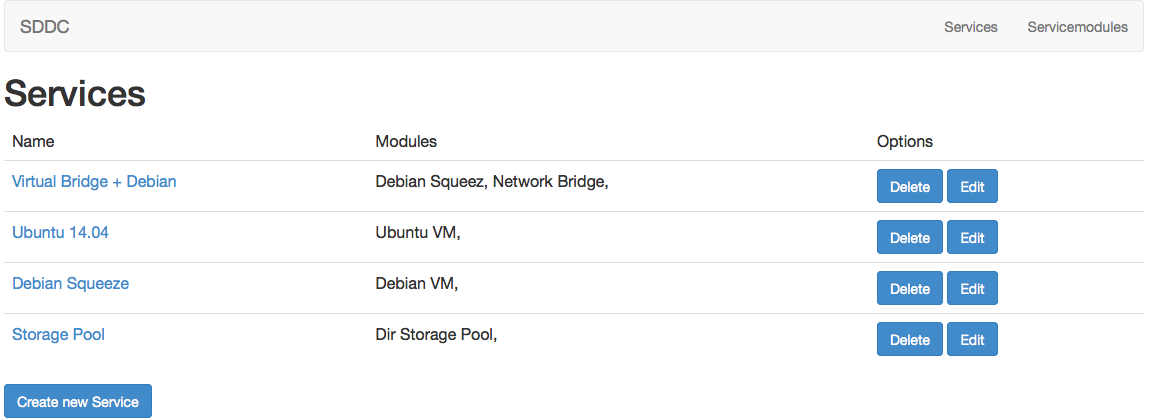
\includegraphics[width=\textwidth]{dashboard}

\end{document}